% %% LyX 1.6.7 created this file.  For more info, see http://www.lyx.org/.
%% Do not edit unless you really know what you are doing.
\documentclass[english,journal=jctcce,manuscript=article,layout=twocolumn]{achemso}
\renewcommand{\familydefault}{\rmdefault}
\usepackage[T1]{fontenc}
\usepackage[latin9]{inputenc}
\usepackage{color}
\usepackage{textcomp}
\usepackage{amsthm}
\usepackage{amsmath}
\usepackage{graphicx}
\usepackage{amssymb}
\usepackage{esint}
\usepackage{multirow}
\usepackage{subcaption}
\usepackage[final]{changes}

\makeatletter

\usepackage[version=3]{mhchem}

%% Because html converters don't know tabularnewline
\providecommand{\tabularnewline}{\\}

%%%%%%%%%%%%%%%%%%%%%%%%%%%%%% User specified LaTeX commands.
%%%%%%%%%%%%%%%%%%%%%%%%%%%%%%%%%%%%%%%%%%%%%%%%%%%%%%%%%%%%%%%%%%%%%
%% This is a (brief) model paper using the achemso class
%% The document class accepts keyval options, which should include
%% the target journal and optionally the macuscript tye
%%%%%%%%%%%%%%%%%%%%%%%%%%%%%%%%%%%%%%%%%%%%%%%%%%%%%%%%%%%%%%%%%%%%%


%%%%%%%%%%%%%%%%%%%%%%%%%%%%%%%%%%%%%%%%%%%%%%%%%%%%%%%%%%%%%%%%%%%%%
%% Place any additional packages needed here.  Only include packages
%% which are essential, to avoid problems later.
%%%%%%%%%%%%%%%%%%%%%%%%%%%%%%%%%%%%%%%%%%%%%%%%%%%%%%%%%%%%%%%%%%%%%
\usepackage[version=3]{mhchem}% Formula subscripts using \ce{}
%%%%%%%%%%%%%%%%%%%%%%%%%%%%%%%%%%%%%%%%%%%%%%%%%%%%%%%%%%%%%%%%%%%%%
%% If issues arise when submitting your manuscript, you may want to
%% un-comment the next line.  This provides information on the
%% version of every file you have used.
%%%%%%%%%%%%%%%%%%%%%%%%%%%%%%%%%%%%%%%%%%%%%%%%%%%%%%%%%%%%%%%%%%%%%
%%\listfiles
%%%%%%%%%%%%%%%%%%%%%%%%%%%%%%%%%%%%%%%%%%%%%%%%%%%%%%%%%%%%%%%%%%%%%
%% Place any additional macros here.  Please use \newcommand* where
%% possible, and avoid layout changing macros (which are not used
%% when typesetting).
%%%%%%%%%%%%%%%%%%%%%%%%%%%%%%%%%%%%%%%%%%%%%%%%%%%%%%%%%%%%%%%%%%%%%
\newcommand*{\mycommand}[1]{\texttt{\emph{#1}}}

%%%%%%%%%%%%%%%%%%%%%%%%%%%%%%%%%%%%%%%%%%%%%%%%%%%%%%%%%%%%%%%%%%%%%
%% Meta-data block
%% ---------------
%% Each author should be given as a separate \author command.
%%
%% Corresponding authors should have an e-mail given after the author
%% name as an \email command.
%%
%% The affiliation of authors is given after the authors; each
%% \affiliation command applies to all preceding authors not already
%% assigned an affiliation.
%%
%% The affiliation takes an option argument for the short name.  This
%% will typically be something like "University of Somewhere".
%%
%% The \altaffiliation macro should be used for new address, etc.
%%%%%%%%%%%%%%%%%%%%%%%%%%%%%%%%%%%%%%%%%%%%%%%%%%%%%%%%%%%%%%%%%%%%%
\author{Mat\'ias A. Nitsche}
\affiliation{Departamento de Computaci\'on, FCEN, UBA, Argentina}

\author{Manuel Ferreria}
\affiliation{Centro de Simulaci\'on Computacional para Aplicaciones Tecnol\'ogicas, CSC, CONICET, Argentina}

\author{Esteban E. Mocskos}
\affiliation{Centro de Simulaci\'on Computacional para Aplicaciones Tecnol\'ogicas, CSC, CONICET, Argentina}
\alsoaffiliation{Departamento de Computaci\'on FCEN-UBA}

\author{Mariano C. Gonz\'alez Lebrero}\email{mcgl@qb.ffyb.uba.ar}\affiliation{Instituto de Qu\'imica y Fisicoqu\'imica Biol\'ogicas, IQUIFIB, CONICET, Argentina}

%%%%%%%%%%%%%%%%%%%%%%%%%%%%%%%%%%%%%%%%%%%%%%%%%%%%%%%%%%%%%%%%%%%%%
%% The document title should be given as usual
%% A short title can be given as a *suggestion* for running headers.
%%%%%%%%%%%%%%%%%%%%%%%%%%%%%%%%%%%%%%%%%%%%%%%%%%%%%%%%%%%%%%%%%%%%%
\title{A GPU accelerated implementation of DFT for hybrid QM/MM simulations.}

\@ifundefined{showcaptionsetup}{}{%
 \PassOptionsToPackage{caption=false}{subfig}}
\usepackage{subfig}
\makeatother

\usepackage{babel}


% \definechangesauthor[name={Mariano C. Gonzalez Lebrero}, color=blue]{MCGL}

\begin{document}
\begin{abstract}
The hybrid simulation tools (QM/MM) evolved into a fundamental methodology for studying chemical reactivity in complex environments.
This paper presents an implementation of electronic structure calculations based on density functional theory (DFT). 
This development is optimized for performing hybrid molecular dynamics simulations by making use of graphic processors (GPU) for the most computationally demanding parts (exchange-correlation terms). 
The proposed implementation is able to take advantage of modern GPUs achieving acceleration in relevant portions between $20$ to $30$ times faster than the CPU version. 
The presented code was extensively tested, both in terms of numerical quality and performance over systems of different size and composition.
\end{abstract}
\maketitle

\section{Introduction}

The simulation of chemical properties in complex systems (solution, proteins, etc.) with electronic detail generally requires treatment by means of computationally expensive methods. 
One approach consists in treating these systems using hybrid (QM/MM) methods. 
In this approach the system is divided into a subsystem treated with a Hamiltonian based on quantum mechanics while the rest is modeled with a classical Hamiltonian. 
This methodology allows for the treatment of complex systems with many degrees of freedom. 
However, the computational cost associated with the resolution the self-consistent electronic problem remains a major constraint when applying this type of model.

Nevertheless, given the immense computing capabilities of the current graphics processing units (GPU), these appear as attractive alternatives in the area of high-performance computing. 
In particular, the use of GPUs in quantum-chemistry has allowed to obtain interesting results. 
There are several works that employ GPUs in diverse electronic-structure calculations~\cite{yasuda_anterior,vogt,ufimtsev,genovese2009density,gpumd,anderson,Skylaris2013}, and there is even a commercial software developed exclusively for this kind of hardware~\cite{Petachem}. 
A particularly relevant work is Yasuda's~\cite{yasuda2008accelerating}, in which an algorithm for the exchange-correlation calculations related to self-consistent field iterations (SCF) is presented. 
It is important to take into consideration that the possibility of obtaining efficient algorithms depends strongly, aside from the hardware to be used, on the type of system that have to be solved (size, type of atoms, basis-functions, etc.).

In our case, it is of great interest the use of hybrid simulation techniques (QM/MM) to study bio-molecules active sites: the presented implementation is oriented towards these systems, which usually are not bigger than $50$ or $100$ atoms and may include relatively heavy elements such as Iron, Sulfur, Copper, etc. \cite{capece2006heme,crespo2003dft,crespo2005multiple,crespo2005theoretical,friesner2005ab,marti2004qm,ridder2003ab,sproviero2006qm}.
Molecular dynamics simulations involve performing complete DFT calculations a large number of times, each with only a few iterations. 
This implies that the initialization time has a greater relative weight in this kind of calculation than in a single-point SCF computation.

In summary, we propose a GPU implementation oriented towards QM/MM molecular dynamics calculations focused on the most computationally demanding steps of a DFT calculation with Gaussian basis. 
This work is based on the code Molecole~\cite{molecole} and include novel approaches having a positive impact on parallelization and performance without affecting numerical quality. 
One of these differences consists in including a new partitioning strategy for the set of quadrature points, which results in a more efficient grouping of computational batches in terms of performance and significative functions. 
Another aspect involves using a low-cost classification criteria for determining these significative functions, which does not require computing the actual function values. 
While other implementations~\cite{yasuda} proposed the recalculation of function values several times at each iteration, in our implementation we precompute these, obtaining notable performance improvements. 

A CPU implementation was also developed and compared to the GPU version.
The CPU version is not simply a translation of the GPU implementation since specific CPU features (like SSE4.1/4.2 or AVX) were used to obtain the best performance possible. 
Finally, we present and test a hybrid code made by the coupling of our DFT implementation with AMBER 12~\cite{Amber12}.

\section{Method}

In the DFT approach, the energy is written as a functional of the density:

{\footnotesize \begin{equation}
E[\rho]=T_{s}[\rho]+V_{ne}[\rho]+\frac{1}{2}\int\int\frac{\rho(\vec{r}_{1})\rho(\vec{r}_{2})}{r_{12}}d\vec{r_{1}}d\vec{r}_{2}+E_{xc}[\rho]\label{eq:DFT}\end{equation}
}{\footnotesize \par}
where the first term is the kinetic energy associated with the density, the second is the interaction between the density and the nuclei, the third one is the Coulombs repulsion of the density with itself and the last is the exchange and correlation energy~\cite{kohnsham}.

The global exchange-correlation portion is the most expensive in terms of computational cost. 
The energy corresponding is calculated by the integral of the local exchange-correlation energy as: 
\begin{equation}
E_{XC}=\int\rho(r)\epsilon_{xc}(\rho(r))dr\label{xc}
\end{equation}
Equation~\ref{xc} can be computed as a discrete sum over a grid~\cite{becke}: 
\begin{equation}
E_{XC}\cong\sum_{j}\rho(r_{j})\epsilon_{xc}(\rho(r_{j}))\label{sum}
\end{equation}
where the electronic density $\rho$ over each grid point $j$ is defined from the molecular orbitals $\psi_{i}$ as: 
\begin{equation}
\rho(r_{j})=\sum_{i}|\psi_{i}(r_{j})|^{2}\label{rho}
\end{equation}
with \begin{equation}
\psi_{i}(x,y,z)=\sum_{k=1}^{n}c_{i}^{k}\chi_{k}
\end{equation}
where $c_i$ are the variational coefficients, and the orbitals $\psi_i$ are constructed by expanding them in a basis of contracted Cartesian Gaussian functions as: 
\begin{equation}
\chi_{k}=(x-x_{0})^{n_{x}^{k}}(y-y_{0})^{n_{y}^{k}}(z-z_{0})^{n_{z}^{k}}\sum_{j}k_{j}^{k}e^{-\alpha_{j}(\vec{r}-\vec{r_{0}})^{2}}
\end{equation}
where 
\begin{equation}
(\vec{r}-\vec{r_{0}})^{2}=(x-x_{0})^{2}+(y-y_{0})^{2}+(z-z_{0})^{2}
\end{equation}

An alternative way to compute the electronic density is using the density matrix:
\begin{equation}
\rho(\vec{r})=\sum_{i=1}^{m}\sum_{j\geqq i}^{m}p_{ij}\chi_{i}(\vec{r})\chi_{j}(\vec{r})\label{eq:density matrix}
\end{equation}
where $m$ is the number of basis functions (or basis functions with a
non negligible value) and:

\begin{equation}
p_{ij}=\sum_{k=1}^{n}C_{i}^{k}\times C_{j}^{k}
\end{equation}
where $n$ is the number of occupied orbitals.

The computation of the exchange and correlation energy (and the corresponding Khon-Sham matrix elements) involves several steps, for all of which a linear-scaling algorithm exists. 
Still, all steps exhibit a degree of parallelism inherent to their mathematical formulation.
Exploiting this aspect gives a notable advantage over sequential procedures.
Nevertheless, there is not a well-established parallel implementation since the computation can be resolved in different ways.
One possible solution consists in parallelizing these steps independently and determining the most adequate parallelization strategy for each one. 
In relation with the diagram shown in Figure~\ref{Flo:esquema}, the main computational steps are: (a) quadrature-point positions, (b) quadrature-point weights, (i) function values, (j) density at each point and (k) Kohn-Sham matrix elements.

To achieve a linear-scaling implementation, Stratman et. al. propose several strategies~\cite{Stratmann1996213}. 
The main idea consists in grouping quadrature-points instead of solving the computation for each one. 
This grouping allows determining which basis-functions have a significative contribution to the final computation, which are referred to as \emph{significative functions}. 
Given the rapid decay of Gaussian functions, the size of the set of significative functions associated with each group of quadrature points does not depend on the number of atoms of the system. 
In other words, this size has constant order in terms of computational complexity. 
As a consequence, it is possible to sub-divide the complete DFT calculation by computing each of these groups independently. 

A simplified scheme of the calculation procedure is shown in Figure~\ref{Flo:esquema}. 
The steps (a) to (e) corresponds to the initialization stage, they are computed once at the start of simulation.
The SCF iteration is composed by steps (f) to (l); this cycle is repeated until the density matrix changes less than a previously established tolerance.
The selected steps parallelized to be run in GPU are (b), (i), (j) and (k), which are the most computationally expensive parts of the code.

\begin{figure}
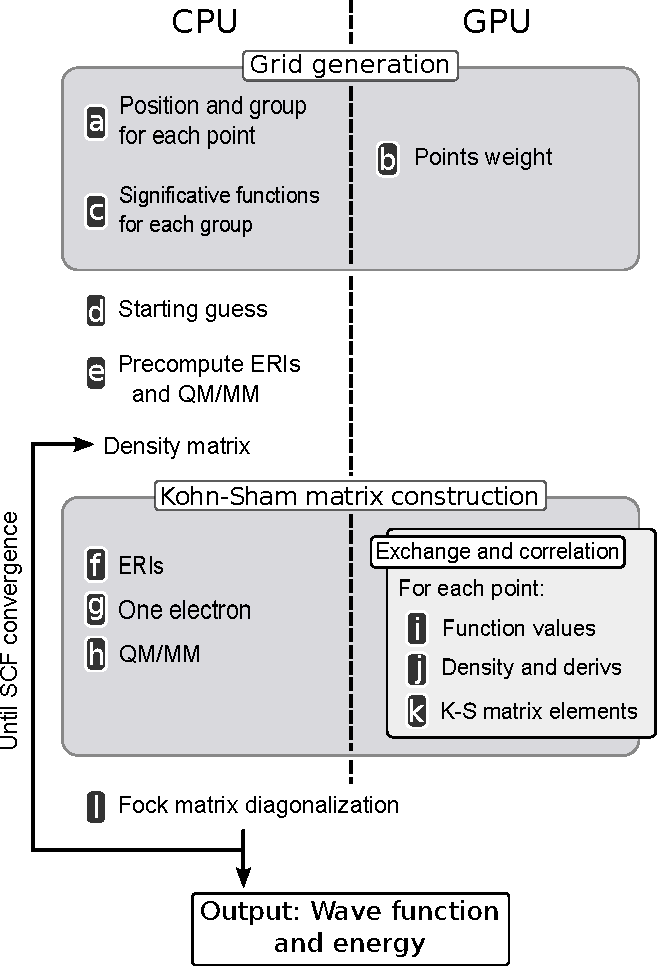
\includegraphics[scale=0.9]{figuras/esquemadecalculobien.pdf}
\caption{Calculations steps, the white box inside Kohn-Sham matrix construction module is the optimized code for GPU.}
\label{Flo:esquema}
\end{figure}

\subsection{The grid}

An important aspect of the calculation is the shape of the grid on which Equation~\ref{sum} is applied. 
The usual practice is to generate a grid for the molecule via atomic overlapping grids. 
These atomic grids come from the superposition of layers derived by scaling a reference layer (see Figure~\ref{Flo:grilla}).

\begin{figure}
\centering
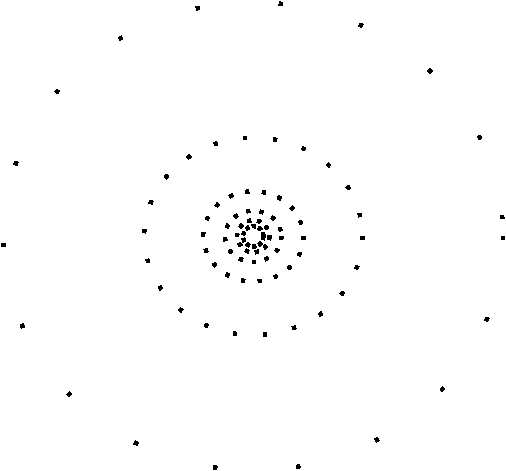
\includegraphics[keepaspectratio,width=0.3\textwidth]{figuras/grilla}
\caption{Schematic atomic grid: layers are not equidistant but are most concentrated close to the nuclei.}
\label{Flo:grilla}
\end{figure}

These layers are not equidistant but are most concentrated close to the nuclei (see Figure~\ref{Flo:capas}), where the electron density changes more abruptly, and are more spaced away from them. 
In a molecule the overlap of atomic grids causes that the relative weight of a given point depends on the position of the grid points from other atoms, making the calculation scale quadratically~\cite{becke}.
However algorithms that scale linearly have been developed.~\cite{Stratmann1996213}

\subsection{Partitioning and function selection criteria}

The simplest partitioning scheme consists of dividing the whole system volume into fixed-size cubes, therefore grouping neighboring points.
However, the distribution of points in space is not homogeneous as a result of the grid shape, which concentrates a large number of points near the nuclei where the electronic density changes more (see Figure~\ref{Flo:capas}).

\begin{figure}
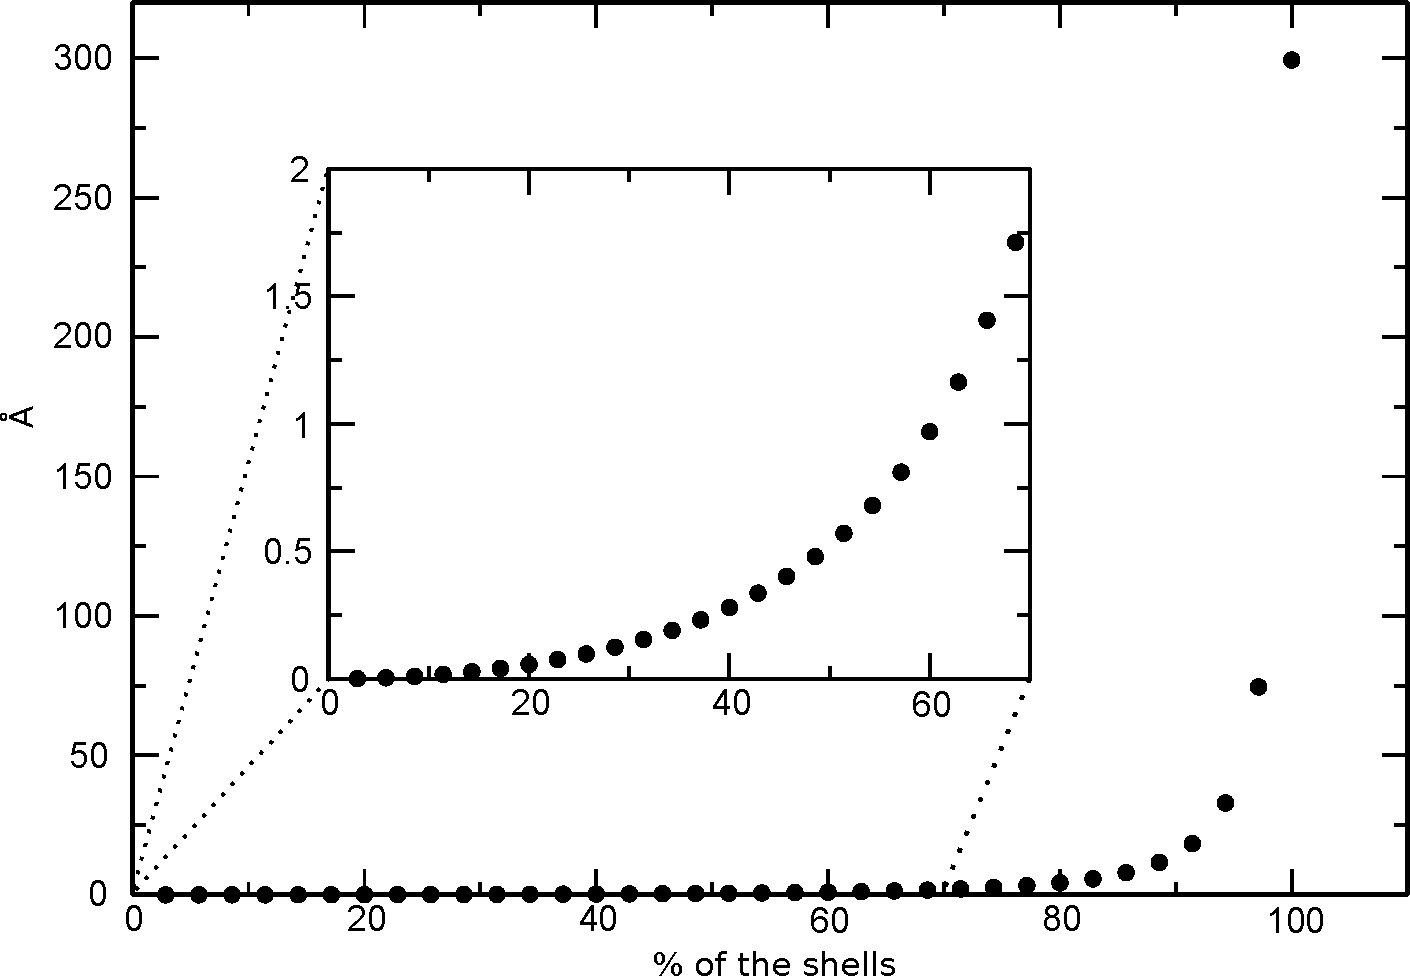
\includegraphics[scale=0.3]{figuras/capas}
\caption{Radii in Angstroms of the grid layers for the oxygen atom.}
\label{Flo:capas}
\end{figure}
These spheres occupy a small space, so there are a reduced amount of significative functions to compute despite having a large quantity of points. 
This produces a reduction in the computational cost, both in GPU as in CPU.
Then, after excluding these already grouped points from the complete point cloud, the traditional cube-based partitioning is applied. 
Using this hybrid partitioning, the cube sizes can be incremented, producing fewer groups.
The result of this hybrid partitioning scheme is a more homogeneous distribution of points in terms of computational cost due to having fewer significative functions in the sphere groups (see \ref{Flo:cubosesferas}).

\begin{figure}
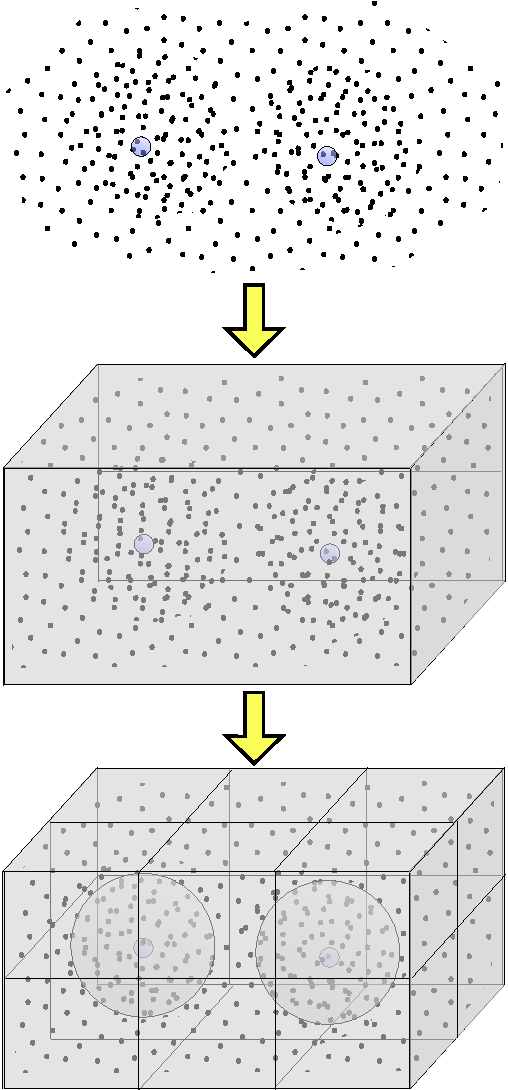
\includegraphics[scale=0.5]{figuras/flowchart}
\caption{Grid partition: combining spheres and cubes (hybrid partition) produces fewer groups and a more homogeneous distribution of points in terms of computational cost.}
\label{Flo:cubosesferas}
\end{figure}

Another optimization implemented in this work consists of a simpler selection criteria for significative functions similar to other packages (for example Gaussian).
Independently of the shape of a group, the selection criteria determines which functions are to be computed over the contained points. 
A simple criteria consist of determining, for each basis function, if the value for that point is greater than a specific threshold $\delta$. 
However, this gives the partitioning and selection criteria a considerable computational cost, since it implies computing all the function values for all points. 
Even further, the cost of computing a basis-function value is not negligible since it involves calculating several Gaussian functions.

The used selection criteria is based on finding a distance of influence for each Gaussian function. 
Outside this radius of influence the function has a negligible value (lower than a parameter: $e^{-\delta}$).
The distance between the Gaussian function center and the group border is calculated, and if the function has a radius of influence larger than this distance the function is discarded.

This condition simplifies the computation by not requiring the actual function value on every point in the group. 
It should be noted that this inclusion condition is only sufficient and not necessary.
This means that some basis functions not meeting this exclusion criteria are still computed but contribute with a negligible value to the calculation. 
Although, the number of these functions is small and do not impact on the resulting computational cost.

As a consequence, with this selection method the computation time for an iteration can be slightly higher than with a more rigorous method but the grid generation time is considerable lower.

\subsection{Computation kernels}

During group partitioning, the positions of the points have to be computed in order to determine in which group they will be contained. 
After the partition is obtained, the list of significative functions of each group is computed. 
These steps (a and c on Figure~\ref{Flo:esquema}) are computed in the CPU, since the corresponding execution time is negligible in both cases. 

The weights of the grid points are computed by a GPU kernel (b on Figure~\ref{Flo:esquema}), since this is the most computational demanding portion of the grid generation step.
This kernel maps one thread to one grid point. 
Shared memory is used as a cache, to store the atom positions and other relevant parameters.

The exchange-correlation calculation in the SCF cycle starts with computing the function values (i on Figure~\ref{Flo:esquema}) in GPU\@. 
Again, one thread is mapped to a single grid point. 
The necessary Gaussian parameters are first loaded into shared memory since these do not depend on the grid point position. 
The function values and their first and second derivatives are stored in GPU global memory in order to be used during the remaining steps of the calculation for each group. 
The size of the memory present in the current GPUs allows storing a great part of these function values (or even all of them) in GPU memory during all the SCF iterations. 
This allows reusing them and drastically diminishes the time of this calculation for the successive steps.
When the next group of points is computed, the value of the functions (and its gradients and Hessians) are recalculated only for the groups that do not have them already stored in GPU global memory.

This approach falls between a fully caching algorithm, where all functions are precalculated and stored for all groups, and a fully recalculating algorithm, where none of the function values are stored but instead are computed on demand for every iteration. 
This latter approach corresponds to Yasuda's work~\cite{yasuda2008accelerating}, where it was shown that the raw processing power of GPUs could be applied in such way to gain significant performance improvements. 
In our case, we took advantage of newer GPU boards which feature faster memory access and increased memory capacity.

The next step of the algorithm consists in computing the density value, the gradient and the Hessian of the density ($j$ on Figure~\ref{Flo:esquema}). 
These steps are the most intensive in terms of floating points operations. 
For this reason, a more detailed explanation of the algorithm is presented.

The calculation performed by this kernel is for all points in the grid using the Equation~\ref{eq:density matrix}. 
The gradient and Hessian are obtained using a similar expression.

\begin{equation}
\rho(point)=\sum_{i=1}^{m}\chi_{i}(point)\sum_{j\geqq i}^{m}p_{ij}\chi_{j}(point)\label{eq:cuentakernel}
\end{equation}
where $m$ is the number of significative functions, $p_{ij}$ is the reduced density matrix, and $\chi_i$ ($\chi_j$) are the values of the $i$ ($j$) function on the considered point.  
The values of the functions ($\chi_j$) are shared for each point, but the density matrix ($p_{ij}$) is different for every pair of functions. 

\begin{figure}
\centering
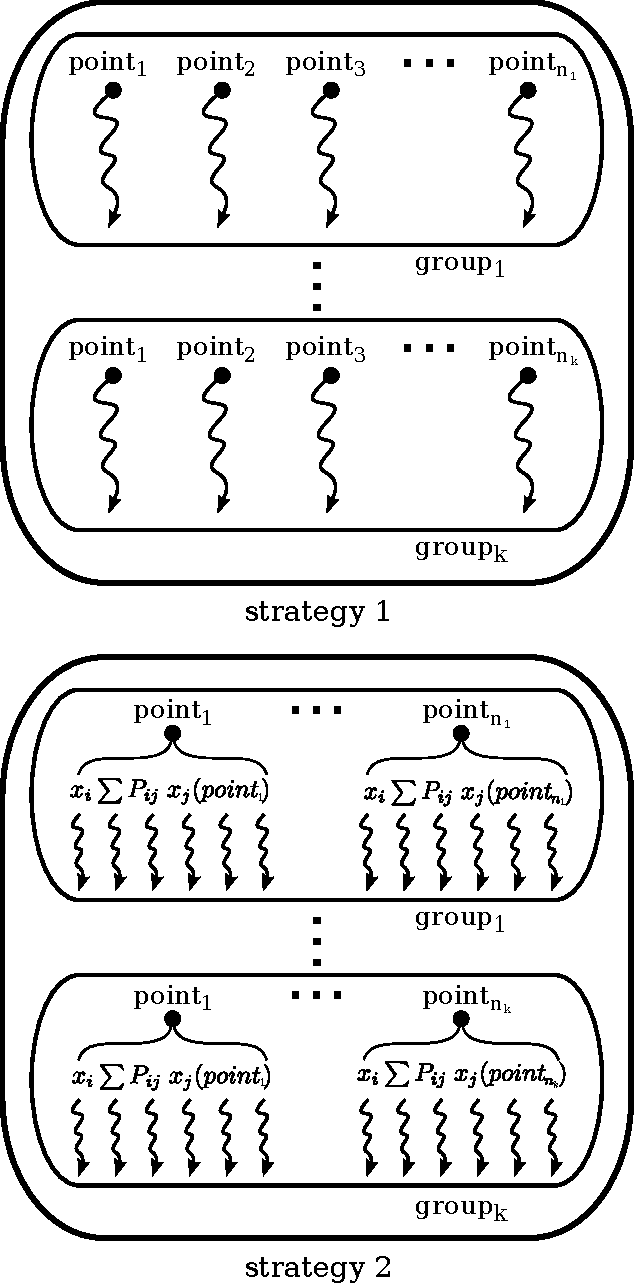
\includegraphics[keepaspectratio,width=0.40\textwidth]{figuras/parallelStrategies}
\caption{Two possible approaches for implementing the step j (Figure~\ref{Flo:esquema}). Strategy 1: point-based parallelization (shares elements of the density matrix, but not the function values and its derivatives). Strategy 2: function-based parallelization (shares the function values but not the density matrix elements).}
\label{Flo:strategies}
\end{figure}

When developing GPU scientific applications, to minimize latency is desirable reusing data reads from global memory as much as possible. 
The dependence of the terms of Equation~\ref{eq:cuentakernel} makes it difficult to do so. 
There are two possible approaches for implementing the step j from Figure~\ref{Flo:esquema}: a point-based parallelization that may share elements of the density matrix, but not the function values and its derivatives (see strategy 1 in Figure~\ref{Flo:strategies}); and a function-based parallelization that can share the function values but not the density matrix elements. 
Initially, a point-based parallelization was implemented, in which each thread computes the entire calculation for a single point. 
However, the performance of this method was not sufficiently acceptable and was discarded.

In the second approach (see Strategy 2 in Figure~\ref{Flo:strategies}), each thread computes two terms $\chi_{i}(point)\sum_{j\geqq i}^{m}p_{ij}\chi_{j}(point)$ corresponding to the Equation~\ref{eq:cuentakernel}; these threads are grouped in an optimal parameter named \texttt{DENSITY\_BLOCK\_SIZE} (\texttt{DBS}, for the current GPU generation the optimal value is $32$). 
A two-dimensional block grid was used, where the $x$ dimension gives the point in the grid and in the $y$ dimension the number of groups of size \texttt{DBS} needed to compute all significative functions. 
Finally, a different kernel performs the summation (i.e. the reduction) over the groups for the same point and computes the contribution to the energy and gradients for that point.

This approach has several advantages. 
Each value of a function, which is shared for all $i$ for the same point, is read only once from global memory to shared memory (in a coalesced form) and is used $2\times $\texttt{DBS} times without bank conflicts. 
The density matrix elements which depends on both $i$ and $j$ are accessed using texture memory\footnote{The texture memory is a specialized cache that allows efficient access to global memory following a tile pattern.}.
This allows fast retrieval of the density matrix elements for close enough $i$ and $j$ (depending on the size of available texture memory). 

The Kohn-Sham matrix contribution is computed using a different kernel, which is necessary during convergence of the main SCF algorithm (step k in Figure~\ref{Flo:esquema}). 
In this kernel, a bi-dimensional grid of threads is used, where each one is mapped to a single matrix element. 
Since the matrix is symmetric, half of these threads would remain idle. 
However, since the computation is actually subdivided in blocks of threads, blocks completely contained in the lower-left triangle of the matrix are discarded without computational cost. 
For the blocks laying over the matrix diagonal, dummy computation is performed for the unnecessary threads in order to minimize branch divergence.
In this step, precision is of key importance (mainly for the GGA based calculations), double-precision variables are internally used in this kernel.
The rest of the GPU kernels can use single-precision variables without significative impact on the final result.
As a result a mixed precision code are used.


\subsection{The Coulomb Integrals}

Another highly CPU demanding part of the electronic-structure calculations corresponds to the Coulomb integrals, which account for the repulsive interaction between electrons (ERIs, third term in Equation~\ref{eq:DFT} and step f in Figure~\ref{Flo:esquema}).
Previous works have proposed the use of GPU for computing these integrals~\cite{ufimtsev,yasuda_anterior}.
In medium size systems, storing ERIs in RAM memory drastically reduces the calculation time of this term compared with the exchange and correlation. 
Therefore in our code this contribution is computed in CPU and stored in main memory.

In principle, this integral depends on four centers. 
This would imply a complexity of $O(m^{4})$ (see Equation~\ref{eq:density matrix}). 
However, this complexity can be easily reduced. 

In particular, we use two approaches in order to reduce the complexity. 
The first one consists in re-writing the density as a linear combination of Gaussian functions (instead of a product of Gaussians) by employing auxiliary basis-functions. This reduces the complexity by one, while also reducing the pre-exponential factor (in general, the number of necessary functions is much lower than the number of products associated with the original basis). 
The second approach for reducing the complexity without compromising the numerical quality consists in employing the \emph{Gaussian Product Theorem}~\cite{Stratmann1996213} to discard negligible terms. 
By using these techniques, a great reduction in the number of terms to compute is achieved.
The obtained complexity is $O(m \times m')$, where $m'$ is the number auxiliary basis functions.
Then, other optimization are applied.
Using the same criteria based on Gaussian product theorem, the coulomb integrals can be classified in two groups depending of its absolute value, the group with the smaller values can be stored using single precision with a negligible loss of accuracy.
The second group (corresponding to the larger absolute values) is stored using double precision.
This optimization reduces the size of the storage needed for this terms.

All these optimizations allows to precompute and store these terms in memory (for example, the Valinomycin (\ce{C54H90N6O18}) with the DZVP basis uses only $5$ GB of memory). 
As a consequence, the time consumed by this portion of the calculation is drastically reduced resulting considerable less than the time involved in the exchange-correlation integral computation.

\subsection{QM/MM implementation}

The DFT GPU based code developed in our group was coupled with the AMBER 12\cite{Amber12} (and AMBER 11) molecular dynamics package.
The periodic boundary conditions were treated with a simple cut-off scheme.
Minor changes on the AMBER code were performed, in particular the possibility of uncoupling the temperature control for the QM and MM subsystems. 
The coupling was made as external program adapting the routines written by Andrea G\"otz and Ross Walker~\cite{walker}.
This implementation was already used in the determination of the free energy profile of the oxidation of cisteine by peroxinitrite.~\cite{Zeida201381}


\section{Results}

Two main aspects are analyzed in the present work: performance and numerical quality. 
In terms of performance, the scalability of the exchange-correlation computation, the overall DFT iteration and
grid generation times are considered. 
Comparisons are performed using GPU and CPU implementations.

The CPU and GPU versions are compared over three different systems of moderate size: Taxol (\ce{C47H51NO14}), Valinomycin (\ce{C54H90N6O18}); and a Heme group without any lateral chains and bound to carbon monoxide (\ce{FeC23N6H16CO}), see Figure~\ref{Flo:molecules}. 
The former two molecules are commonly used in performance measurements~\cite{yasuda2008accelerating,PetachemResults}, and the latter is a typical example of a system that is studied using hybrid techniques~\cite{capece2006heme,crespo2005theoretical}. 
For all cases, we employs the DZVP basis set with a DGA1 auxiliary basis set. Computations are performed using a high-density grid ($194$ angular points and $30$ to $35$ shells). 
The PBE~\cite{PBE} functional was adopted for all the calculations.

\begin{figure*}
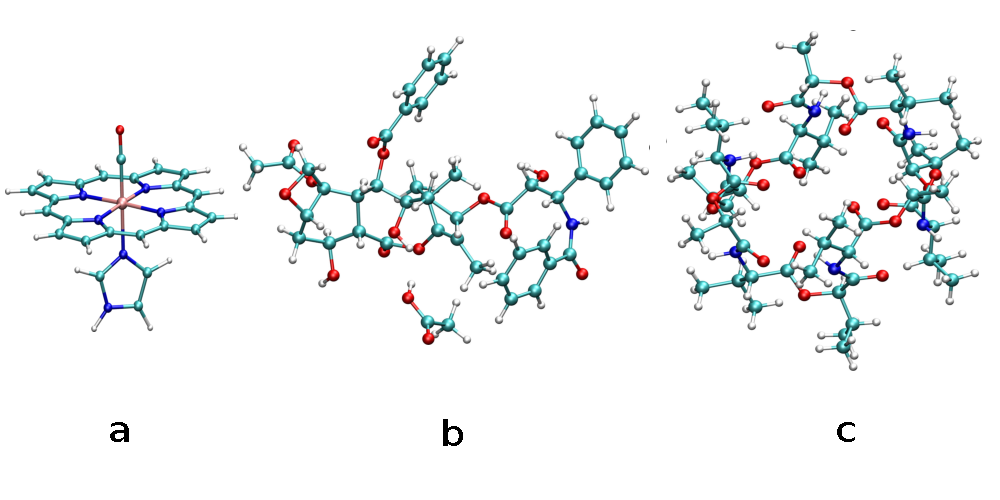
\includegraphics{figuras/moleculas}

\caption{Schematic representation of the systems used to test the implementations: a) Heme group without any lateral chains and bound to carbon monoxide (\ce{FeC23N6H16CO}), b) Taxol (\ce{C47H51NO14}), c) Valinomycin (\ce{C54H90N6O18}).}
\label{Flo:molecules}
\end{figure*}

\subsection{Technical details}

The graphical processor used for the tests is NVIDIA\textregistered{} GeForce GTX 780, implementing the Kepler architecture and having 3GB of DDR5 graphical memory.
This GPU was installed on a desktop PC with an Intel\textregistered Core\texttrademark{} i5-3330 processor (3.0GHz clock speed and 6MB cache size) and 8GB of memory.
The CPU based implementation is tested in the same desktop PC.

The GPU implementation uses CUDA\texttrademark{} (Compute Unified Device Architecture), which is a parallel computing platform and programming model created by NVIDIA\textregistered. 
The GPU Computing SDK used is the CUDA\texttrademark{} Toolkit Version 5.5, which is bundled with the driver version 319.60, which includes the necessary run time libraries and compiler.

Both CPU and GPU implementations are specifically optimized for the corresponding architecture. 
In the case of the CPU version, it consisted in a sequential version using Floating-point vector library (\texttt{fvec}, developed by Intel\textregistered) producing \texttt{SSE2} type instructions.

The parallelized version of Math Kernel Library (\texttt{MKL}, developed by Intel\textregistered) is used for certain steps that are solved in both implementations in CPU (for example matrix diagonalization).

\subsection{Numerical Quality}

Two aspects mainly affect the numerical quality, the parameter $\delta$ and the use of mixed precision in the exchange correlation terms.
Table \ref{calidad} shows the final energy and differences for two set of parameters on the systems presented in Figure \ref{Flo:molecules}.
In the first one, the computation is done using a CPU version without discarding any functions and exclusively using double precision. 
The second one is based on a GPU version with $\delta=10$ and mixed precision.
These results show in all cases a difference bellow of $1$ kcal/mol (``chemical accuracy''), concluding that are equivalent.

\begin{table}
\scriptsize
\begin{minipage}{0.45\textwidth}
\renewcommand{\arraystretch}{1.5}
\centering
 \begin{tabular}{c|c|c|c}
   &Heme & Taxol & Valinomicin \\
\hline
 CPU\footnote{With full double precision and without discarding any function.}  & $-1625197.143$ & $-1835014.862$ & $-2378314.553$ \\
 GPU\footnote{With $\delta=10 $ and using mixed precision.} & $-1625197.125$ & $-1835014.764$ & $-2378314.264$ \\ 
diff & 0.018 & 0.098 & 0.288 \\
\end{tabular}
\end{minipage}
\caption{Final energy (in Kcal/mol) and differences showing that using a full double precision or a mixed precision and discarding negligible functions produces equivalent results.}
\label{calidad} 
\end{table} 

After determining $\delta$, the sizes of the cubes and the shells included in the spheres should be optimized.
The optimal parameters found for maximizing performance on GPU and CPU are different. 
Both cases share the same percentage of shells in the spherical groups ($60\%$), but the size of the cubes are significantly different (CPU: $1$a.u., GPU: $8$a.u.). 
The cube size is strongly related with the total computational cost. 
The selection of functions to be dropped is more effective with smaller cubes, reducing the number of functions and points in each one. 
For CPU, having large quantities of groups with small computational cost is a desirable scenario, being only limited by the available memory.
In GPU, where a large amount of processing cores is available (e.g.\ the Nvidia GTX $780$ has $2304$ CUDA cores), this situation results in less efficient computation.
For this reason, is normally preferred having larger cubes in despite of increasing the computational cost.

\subsection{Scalability Analysis}

One important aspect to verify is the linear scalability of this implementation with respect to the number of atoms. 
Execution times for the exchange-correlation calculation were measured for the GPU implementation. 
This was done on systems consisting of a series of water clusters of growing size ($1-24$ molecules) with a DZVP basis-set and an auxiliary DGA1 basis-set. 
The quadrature grids of tested have~\cite{lebedev1,lebedev2,becke}: $194$ angular points, and $30$ to $35$ shells (depending on the element). 
The DFT-GGA functional PBE was used.

\begin{figure}
\centering
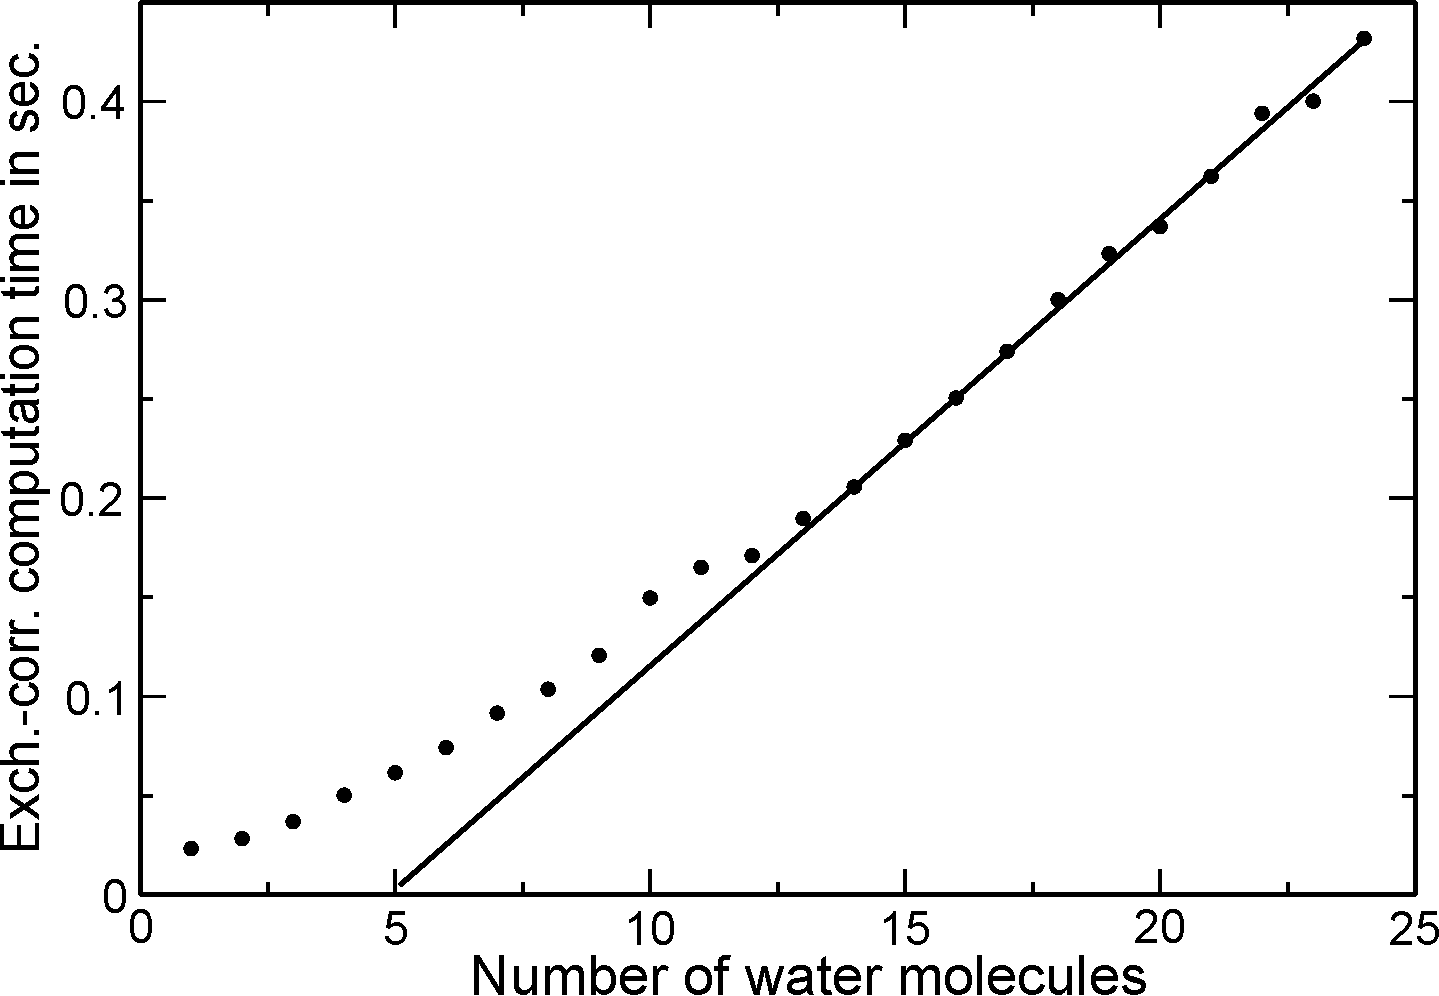
\includegraphics[scale=0.33]{figuras/escalamiento}
\label{Flo:scalability}
\caption{Scalability analysis: best times obtained for high density grids for the water clusters systems.}
\end{figure}



\subsection{Performance}

\subsubsection{Group partitioning}

The use of a hybrid group partitioning scheme based on spheres surrounding the atoms and cubes for the rest of the points have a positive impact on performance. 
In Table~\ref{tablaesferas} we show the exchange and correlation execution time with the best parameter with and without the spheres groups, for the Heme and Valinomycin (both with DZVP basis set).

In all cases the impact is similar, and the execution time is decreased by $33$ to $37\%$ without loss of accuracy in GPU (in CPU have similar results) implementation.
The best results are obtained using a value between $50$ and $70\%$ of the grid points for the spheres.

\begin{table}
\begin{tabular}{c|ccc} 
               & Heme    & Taxol    & Val. \\
\hline
Hybrid partition & 0.55  & 1.40 & 2.55 \\
Cubes only & 0.82 & 2.21 &  3.90 \\
\hline 
Speedup & 33\% & 37\% & 35\% \\
\end{tabular}
\caption{Execution Times (in seconds) for exchange-correlation terms for different partition schemes \added{in GPU}. The use of hybrid partition presents a speedup of near $35\%$ in the considered systems.}
\label{tablaesferas}
\end{table}

\added{In the hybrid partition scheme and using the presented parameters for GPU, the number of significative functions per group varies from only a few to more than $800$ (using valinomicine as an example). 
However the total time is strongly dominated by the groups with more than $256$ significative functions. 
Those groups consume more than 90\% of the total computing time.}

\subsubsection{Performance Considerations}

The available GPU cards present an impressive theoretical computing power, for example the GeForce GTX 780 can process $4$ TFLOPS (peak performance) in single precision.
However real applications have several limitations to achieve this outstanding performance. 
Examples of limitations are the need of synchronization and acceding data from memory. 

One of the paradigmatic applications in scientific computing is matrix computation. 
The NVIDIA\textregistered CUDA Basic Linear Algebra Subroutines (cuBLAS) library is a GPU-accelerated version of the complete standard BLAS library~\cite{cublas}.

The different matrix operations show a strong variation in terms of obtained performance.
For example, \texttt{SGEMM} obtains $2779$ GFLOPS while the symmetric version \texttt{SSYMM} only performs $876$ GFLOPS (data taken from Nvidia Performance Report~\cite{cublasReport}) using K20X board with cuBLAS 5.0.
This reveals the variations even in testbed scenarios focused on operations with large matrices.

In our application, the most demanding kernel corresponds to computing the density (gradient and Hessian) on each point. 
The number of terms to compute the equation~\ref{eq:density matrix} are given by:

\begin{equation}
\#_{terms}=\dfrac{1}{2} \sum_{groups}\#_{points}\#_{fcts}\times \left(\#_{fcts}+1\right)
\end{equation}
Where  $\#_{points}$ are the number of points in the group and $\#_{fcts}$ are the number of significative functions for this group.
In the larger case (Valinomicin with DZVP basis set) the number of such terms are $4.40\times10^{11}$.
The number of floating points operation for computing each term have a minimum of two (one multiplication plus one accumulation), discarding the reading from local, texture and shared memory, dummy computation etc.
The time needed to compute these terms in a GeForce GTX 780 is $1.37$ sec, leading to a result of $640$ GFLOPS. 
This performance is similar to that achieved by the CUBLAS \texttt{SSYMM} in a Tesla K20x GPU~\cite{cublasReport}, a much powerful board. 

\subsubsection{GPU vs CPU}

\begin{table*}
\footnotesize

\begin{minipage}{\textwidth}
\begin{center}
\renewcommand{\arraystretch}{1.5}


\begin{tabular}{cl|ccccc}

 & & GPU & CPU$_1$\footnote{With the same parameter as GPU.} & CPU$_2$\footnote{With the best parameters for CPU.} & CPU$_1$/GPU & CPU$_2$/GPU \\
\hline
\hline
\multirow{3}{.8cm}{Heme} & Grid gen                  & 0.304    &   6.782  &  8.438     &  \textbf{22}   & \textbf{28} \\
                        & SCF                        & 1.021    &  25.822  & 16.551     &  \textbf{25}   & \textbf{16} \\
                        & \hspace{0.3cm} Exc-corr    & 0.549 	&  25.474  & 16.094 	&  \textbf{46}   & \textbf{29} \\
\hline
\multirow{3}{.8cm}{Taxol} & Grid gen                 &  0.868 &  30.775  &   25.503   &    \textbf{35}  & \textbf{29} \\
                        & SCF                        &    4.246  &  72.562   &  40.028    &   \textbf{17}   & \textbf{9} \\
                        & \hspace{0.3cm} Exc-corr    &  1.395    &  69.077    & 36.433     &   \textbf{50}   & \textbf{26} \\
\hline
\multirow{3}{.8cm}{Val.} & Grid gen                 &   1.637  &   72.247  &    43.042  &  \textbf{44}  &  \textbf{26} \\
                          & SCF                      & 10.566     &  133.99   & 62.605     &  \textbf{13}  &  \textbf{6} \\
                          & \hspace{0.3cm} Exc-corr  & 2.317 & 125.350 & 53.019 &   \textbf{54}   & \textbf{23} \\

\end{tabular}

\end{center}
\end{minipage}

\caption{GPU and CPU performance comparison for selected systems for one SCF iteration. Times are in seconds.}
\label{comparacion}
\end{table*}

The Table~\ref{comparacion} includes a comparison of execution times for an iteration of the SCF calculation for Heme, Taxol and Valinomicin with a DZVP basis set and DGA1 auxiliary basis set.

The overall performance is similar to the well known ORCA package (version 2.9.1).
Using this package, the time for an iteration using exactly the same basis, auxiliary set and a similar number of grid points is: $23.53$s for Heme,  $65.30$s for Taxol and $122.39$s for Valinomicin.
Despicte that the computation is not exactly the same (for example, ORCA does not store ERIs in memory) and ORCA uses more grid points ($40\%$ more in Heme, $30\%$ more in Taxol and $20\%$ more in Valinomicin), this comparison reveals that the used CPU implementation is comparable with the state on the art in the Quantum Chemistry field.

For the CPU case, two sets of parameters are used: CPU$_1$ uses the same parameters than GPU, and CPU$_2$ is computed with optimized parameters for the CPU. 
\added{On both cases, only one core is used for the execution. 
The application is compiled using the available specific compiler optimizations for the current processor architecture.}

Using the best parameters for CPU (CPU$_2$ case) lowers the number of significative functions and thus the number of floating point operations performed. 
In spite of being measuring different workloads, this procedure results a fair comparison of the two computing platforms each one with its best available scenario.

On the other hand, the use of the same set of parameters (CPU$_1$ case) allows to compare the two computing platforms performing exactly the same operations.

In the Table~\ref{comparacion}, the first row of each considered system corresponds to the grid generation stage. 
For the CPU$_1$ case, the speedup ranges between $22$ and $44$ times, showing an increment with the system size.
For the other case, the obtained speedup is near $28$ times in all the considered systems. 

For all considered systems, the exchange-correlation part of SCF iteration represents a large part of its total computing time in both CPU cases. 
For example, in Taxol (CPU$_2$ case) represents more than $90\%$ of the SCF iteration.

When the same amount of operations is performed in each platform (CPU$_1$ case) the obtained speedup for the GPU implementation (column CPU$_1$/GPU in Table~\ref{comparacion}) for the exchange-correlation part ranges between $46$ and $54$ times.
For the CPU$_2$ case, this speedup (column CPU$_2$/GPU) is $23$ times for Valinomicin and $29$ times for Heme.

These results show that use of the GPU implementation produces a drastic reduction in the computing time for the exchange-correlation part of the SCF iteration.

\subsection{QM/MM simulations}

In this section, the impact of the new implementation on a QM/MM simulation is evaluated.
The system used is the soluble domain of CopA ATPase from \textit{Archaeoglobus fulgidus}. 
This protein couples the energy of ATP hydrolysis to \ce{Cu+} translocation across cellular membranes~\cite{Toyoshima}.
In the reaction mechanism a phosphorylated metastable intermediate is generated.
This particular autophosphorylation reaction results in a interesting example of a system that can be studied using QM/MM tecnhiques.

In the QM/MM simulation, the QM subsystem is defined by the atoms in the reactive region. 
This includes the phosphates of the ATP, one Mg$^{2+}$, the aspartic 424 (which is phosphorylated) and some of the atoms of lysine 600; totalizing $34$ atoms (see Figure~\ref{Flo:qmmmsystem}).
The MM subsystem is formed by the rest of the protein, the rest of ATP, explicits waters molecules and \ce{Na+} counterions. 
The initial coordinates are taken from 3A1C structure of the Protein Data Bank (PDB)~\cite{Toyoshima} and relaxed using classical simulation for $2$ns.

\begin{figure}
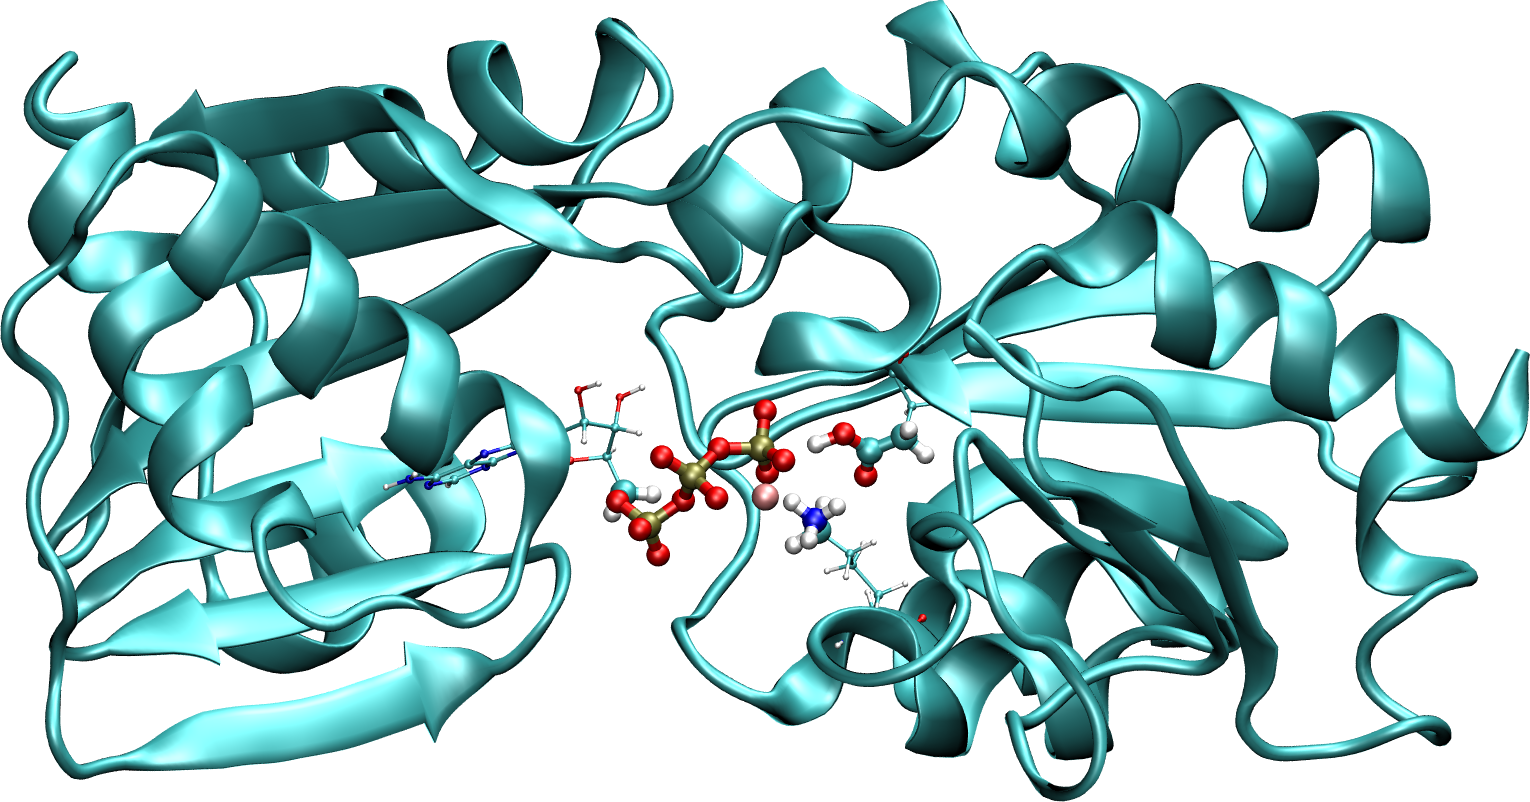
\includegraphics[keepaspectratio,width=0.45\textwidth]{figuras/qmmm.png}

\caption{QM/MM system, the water molecules are not show, the QM region are showed in CPK representation}
\label{Flo:qmmmsystem}
\end{figure}

The Figure~\ref{Flo:ComparacionTiempos} shows the relative times for the one step of molecular dynamics, taking $8$ SCF iterations to converge. 
Figure~\ref{Flo:qm_mm_antes} includes the results for CPU based implementation using the best available parameters while Figure~\ref{Flo:qm_mm_despues} is centered on the GPU version. 

\begin{figure*}[ht]
\centering
\begin{subfigure}[b]{0.48\textwidth}
  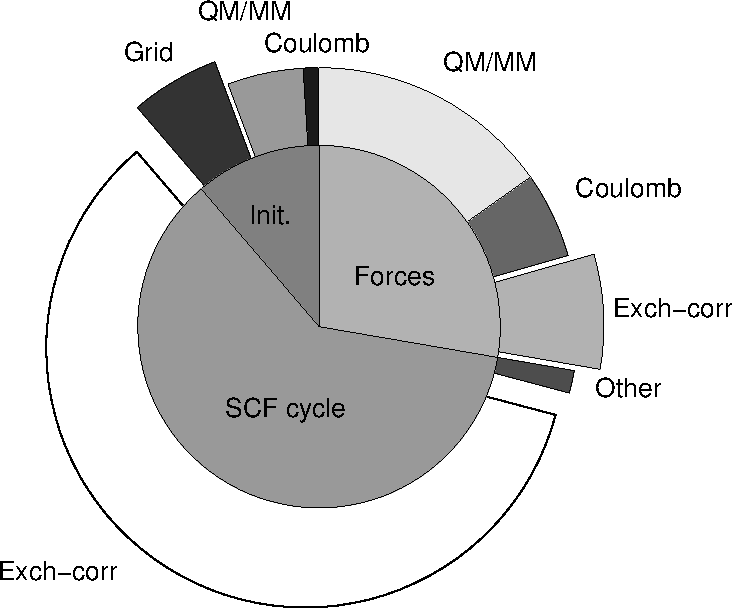
\includegraphics[keepaspectratio, scale=0.65]{figuras/qm_mm_antes.pdf}
  \caption{CPU version, total time $87.52$s}
  \label{Flo:qm_mm_antes} 
\end{subfigure}
\begin{subfigure}[b]{0.48\textwidth}
  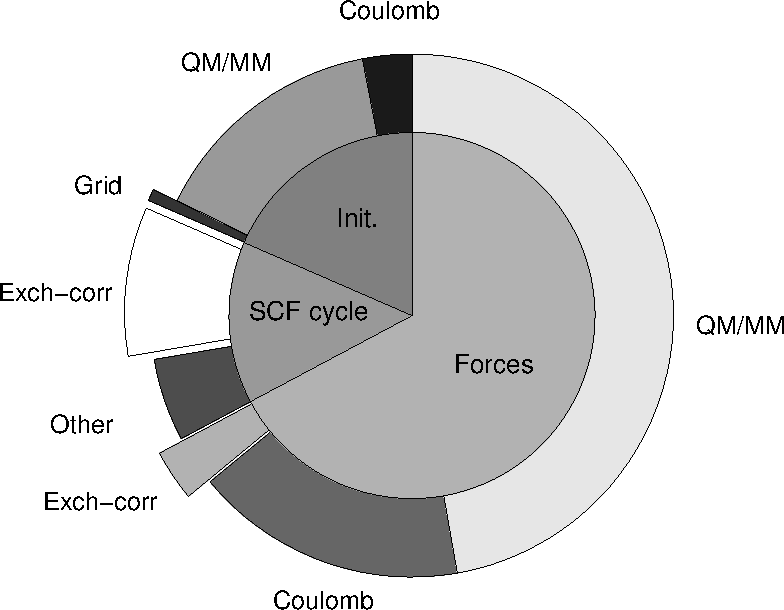
\includegraphics[keepaspectratio, scale=0.65]{figuras/qm_mm_despues.pdf}
    \caption{GPU version, total time $26.56$s}
  \label{Flo:qm_mm_despues} 
\end{subfigure}
\caption{Relative times for one step of molecular dynamics simulation. The emphasized portions correspond to the steps ported to GPU.}
\label{Flo:ComparacionTiempos}
\end{figure*}

As was previously mentioned and can be immediately seen in Figure~\ref{Flo:qm_mm_antes}, the exchange-correlation calculus in SCF cycle is one of the most demanding parts in terms of computational cost. 
On the other hand, the Figure~\ref{Flo:qm_mm_despues} shows that this stage is notoriously diminished in the GPU version, reaching a speedup of 20X.
As a consequence, the relative weight of the exchange-correlation calculus in SCF cycle is bellow QM/MM initialization, QM/MM Forces and Coulomb Forces.
The grid generation stage and the exchange-correlation forces also present a remarkable speedup.
The Figure~\ref{Flo:qm_mm_despues} shows that the relative impact of these two terms in the GPU version is minor. 

\section{Conclusions}

The hybrid simulation tools (QM/MM) evolved into a fundamental methodology for studying chemical reactivity in complex environments.
The aim of this work is to devise an electronic-structure simulation software based on DFT as efficient as possible, in order to be applied to hybrid molecular dynamic simulations. 
In this sense, two particularities of these type of calculations were considered due to their importance: the size of the systems (which usually consist of a moderate number of atoms, on the order of $100$) and the nearness to convergence of the wave function at the first SCF iteration (which minimizes the number of required iterations). 

In the SCF iteration part, the use of an hybrid partitioning scheme reduces the computational cost by $35\%$ and the use of GPU contributes in an additional 20 to 30X factor (compared with the best implementation in CPU using a single core).

Although, the reduction in the time consumed by the exchange-correlation calculus reveals other parts that acquire relevance in the GPU version.
As is shown in Figure~\ref{Flo:qm_mm_despues}, some of the steps that should be considered to further optimization are QM/MM force, Coulomb force, and, to a lesser degree, other terms (Basis changes, Matrix diagonalization, etc).

The obtained results show a successful implementation of the exchange-correlation part of the DFT calculation that can measure up to the state of the art of the field.
This new version also presents optimal characteristics to be included as part of a molecular dynamics simulation software. 


\begin{acknowledgement}
This work was partially supported by the University of Buenos Aires and the CONICET. 
We thanks to A. Roitberg for a generous allocation of computer time, Dar\'io A. Estrin for useful discussions and David Gonz\'alez M\'arquez for his help with the figures. 
\end{acknowledgement}



\bibliography{paper}

% \listofchanges[style=list]

\newpage

\begin{figure*}
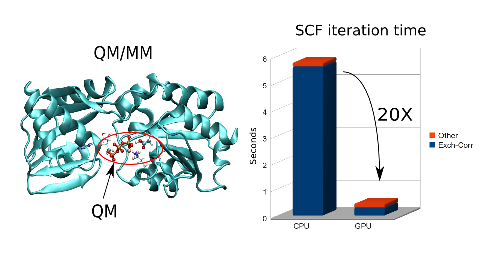
\includegraphics[]{figuras/toc.pdf}
\caption{For table of contents only}
\end{figure*}

\end{document}
